\documentclass[12pt]{article}

\usepackage{paralist}
\usepackage{amsfonts}
\usepackage{amsmath}
\usepackage{hhline}
\usepackage{booktabs}
\usepackage{multirow}
\usepackage{multicol}

\usepackage{graphicx}
\graphicspath{ {images/} }

\oddsidemargin 0mm
\evensidemargin 0mm
\textwidth 160mm
\textheight 200mm
\renewcommand\baselinestretch{1.0}

\pagestyle {plain}
\pagenumbering{arabic}

\newcounter{stepnum}

%% Comments

\usepackage{color}

\begin {document}

\title{\textbf{StormWare}}
\author{Group 15\\ Anirudh Verma\\ David Hospital\\ Sijie Zhou\\ Zijing Chen}
\maketitle

\begin{center}
\rule{7cm}{0.4pt}\\
\thispagestyle{empty}
\parskip=14pt%
\vspace*{3\parskip}%

McMaster University

Department of Computing and Software

COMPSCI 2XB3



\end{center}

\newpage

\tableofcontents


\newpage

\hspace{0pt}
\vfill
\textit{By virtue of submitting this document we electronically sign and date that the work being submitted by all the individuals is the group is their exclusive work as a group and we consent to make available the application developed through CS-2XB3 project, the reports, presentations, and assignments (not including my name and student number) for future teaching purpose.}
\vfill
\hspace{0pt}
\newpage


\section{Team Members and Role Assignment}

\begin{tabular}{| l | l | l |}
\hline
\textbf{Team Members} & \textbf{Student Number }& \textbf{Roles }\\
\hline
Anirudh Verma	&400039737	&Owner \\
\hline
David Hospital	&400015029	&Developer\\
\hline
Sijie Zhou	&400038163	&Quality Assurance\\
\hline
Zijing Chen	&400020376	&Designer\\
\hline
\end{tabular}


\section{Contribution}
\begin{tabular}{|p{3cm}|p{4cm}|p{3cm}|p{5cm}|}
\hline
Name	&Role	&Contribution	&Comment\\
\hline
Anirudh Verma	&Owner	&Parser module	&\\
\hline
David Hospital	&Developer	&Proposal	&\\
\hline
David Hospital	&Developer	&Data and DisasterEvent module	&\\
\hline
Sijie Zhou	&Quality Assurance	&Requirement spec	&\\
\hline
Sijie Zhou	&Quality Assurance	&Presentation slide	&\\
\hline
Sijie Zhou	&Quality Assurance	&Design spec	&\\
\hline
Zijing Chen	&Designer	&MainActivity module	&\\
\hline
All	&Group 15	&Design spec	&The design spec is not finished by an individual. It’s a group effort.\\
\hline
\end{tabular}


\section{Revision History}
\begin{tabular}{|p{3cm}|p{3cm}|p{3cm}|p{5cm}|}
\hline
\textbf{Timestamp} & \textbf{Originator}& \textbf{Version Number } & \textbf{Comment}\\
\hline
180209T1014	&All	& \#1	&Topic selected\\
\hline
180209T1014	&All	&\#1	&Team roles decided\\
\hline
180209T1014	&All	&\#1	&Setup github repo\\
\hline
180209T1014	&All	&\#1	&Implementation platform decided\\
\hline
180216T1107	&All	&\#1	&Create log file\\
\hline
180216T1107	&All	&\#1	&Specification decided: Using google map API and possibly machine learning for data parsing\\
\hline
180228T1405	&All	&\#1	&Completed requirements specification\\
\hline
180302T1100	&All	&\#2	&Start prototype\\
\hline
180302T1100	&All	&\#2	&Discussed prototype design and requirements\\
\hline
180305T0200	&David Hospital	&\#2&	Create Android Studio project and commit it to github repo\\
\hline
180307T1300	&All	&\#3	&Discussed relevance of machine learning and abandon machine learning\\
\hline
180309T1000	&All	&\#3	&Continued work on Parser.java and created Test.java.src/.../Parser.java\\
\hline
180316T1000	&All	&\#3	&Discussed project objective and how much data to display at once\\
\hline
180323T1000	&All	&\#4&	Final version confirmed and requirements modified\\
\hline
\end{tabular}

\newpage
\section{Executive Summary}

The application is an Android mobile program using Google Map API which will help user to have an overall view of natural disasters in America. Users can choose one exact disaster type and the output will show by the form of heatmap.

\section{Internal Evaluation}

Overview: 
In this document we have presented a full report on the work undertaken to design and build the application in response to all the requirements of the stakeholders, and to the specification and plan provided in the brief. 

The application is an Android mobile program using Google Map API which will help user to have an overall view of natural disasters in America. Users can choose one exact disaster type and the output will show by the form of heatmap.
Problems faced and Improvements: 

\begin{itemize}
\item Parser: The parser that we had implemented initially was creating performance issues (it took 24 seconds with our first parser) and we decided to implement a second parser which allowed for faster processing by 80\%. It reduced the loading time to 8 seconds. 
\item Search Bar: For our interface, we decided to implement a search bar which allowed users to search locations and disaster events by type. Following that, the team felt that the user interface needed more functionality, for which we added a horizontal scroll view listing disaster types that can be directly selected to output the heat map, instead of typing the type. We decided to keep the search bar as it allows users to select locations on map as a normal search bar does. 
\end{itemize}

Review Questions:
\begin{itemize}
\item Does it meet the design need or situation? 

Yes, the design needs for the project have been met.
\item Does it fit the purpose for which it is intended? 

Yes, as per our initial planning, we have been able to make a project which covers the needs of our intended user base which includes (but is not limited to) governmental agencies for planning location sensitive things, researchers, weather networks and anyone who would be interested in knowing/working with the history of disaster events in a given area(in the US).
\end{itemize}

Concluding Remarks: The team felt that if time and skill set permitted, we would have gone ahead with integrating machine learning in our project to employ neural networks for processing patterns of disaster events that we are currently displaying in our app. 

\section{UML Class Diagram}
\begin{figure}[h!]
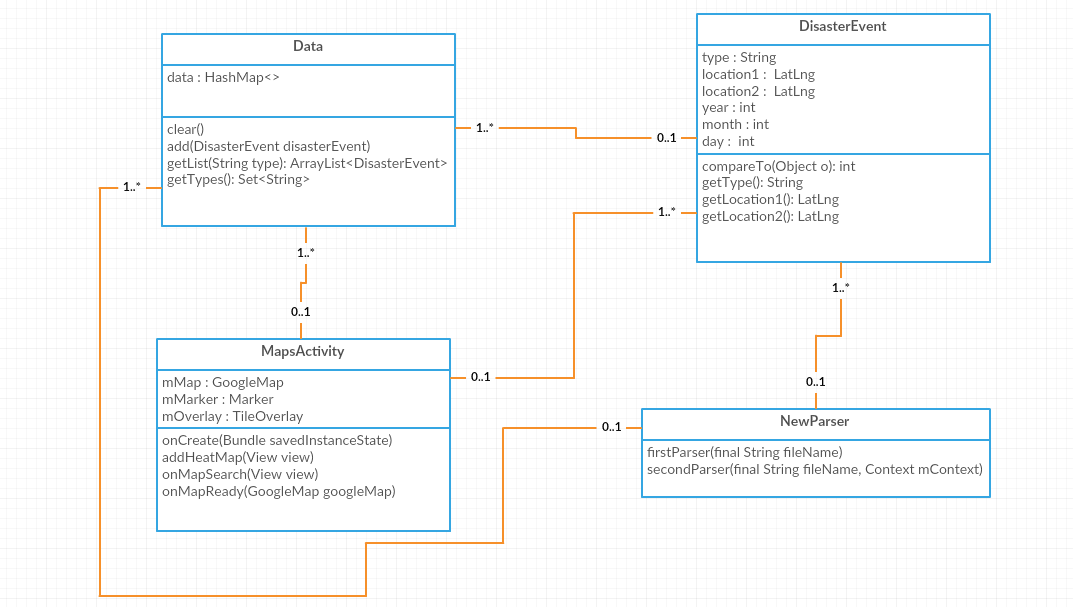
\includegraphics[scale=0.4]{uml}
\caption{\textit{DisasterEvent uses nothing. Data uses DisasterEvent. NewParser uses data and DisasterEvent. MapsActivity uses NewParser, Data and DisasterEvent.}}
\end{figure}

\noindent DisasterEvent:
\begin{itemize}
\item	Module for creating DisasterEvent objects, used to store information about each event.
\item Has start and end location, time (year, month, and day), and event type variables.
\end{itemize}

\noindent Data:
\begin{itemize}
\item Module for Storing and sorting a large collection of DisasterEvent objects.
\item Uses a HashMap to partition events into different lists, separated by their type.
\item Lists can be accessed by using the event type as a key in the HashMap.
\item When a event is added and the HashMap does not contain a list for that type, it creates a new list and appends the event to it.
\end{itemize}

\noindent NewParser:
\begin{itemize}
\item	Module for parsing data from specifically designed csv files directly into the Data module
\item	The method firstParser is responsible for condensing the raw data file with over 40 columns into a smaller file with just 8 columns.
\item	The method secondParser is responsible for parsing the condensed data file and creating a DisasterEvent object for each row. These events are added to the Data module using Data.add.
\item	The parsing time for the secondParser is 80\% faster than firstParser, making it a valuable improvement to the module.
\end{itemize}

\noindent MapsActivity:
\begin{itemize}
\item	Module for handling the controller and view components of the program.
\item	Uses the Android framework as a backbone for handling most of the input and output events.
\item	The onCreate method is called when the program starts and is responsible for loading the google map view onto the screen.
\item	The addHeatMap method is called whenever one of the type buttons is pressed (UI event). It removes the old heatmap object if there is one, and then adds a new one, by getting the list of DisasterEvent objects from the given type from the Data module. It then passes that list to the google map framework to create a heatmap and displays it on the map.
\item	The onMapSearch method is called whenever the user presses the search button (UI event). The text that is currently in the search bar is sent to the google map framework which returns a list of possible addresses that it might match. The first one is picked (best result). A marker is created (the old one is removed) on the map at that result and the camera is translated to focus on the new marker. 
\end{itemize}


\newpage

\section {Disaster Event Module}

\subsection {Module}

DisasterEvent

\subsection {Uses}

LatLng (android)

\subsection {Syntax}

\subsubsection {Exported Types}

DisasterEvent = ?

\subsubsection {Exported Access Programs}

\begin{tabular}{| l | l | l | l |}
\hline
\textbf{Routine name} & \textbf{In} & \textbf{Out} & \textbf{Exceptions}\\
\hline
DisasterEvent & String, LatLng, LatLng, $\mathbb{Z}$, $\mathbb{Z}$, $\mathbb{Z}$ & DisasterEvent & \\
\hline
compareTo & DisasterEvent & $\mathbb{Z}$ & ~ \\
\hline
getType & ~ & String & ~ \\
\hline
getLocation1 & ~ & LatLng & ~ \\
\hline
getLocation2 & ~ & LatLng & ~ \\
\hline
getYear & ~ & $\mathbb{Z}$ & ~ \\
\hline
getMonth & ~ & $\mathbb{Z}$ & ~ \\
\hline
getDay & ~ & $\mathbb{Z}$ & ~ \\
\hline
\end{tabular}

\subsection {Semantics}

\subsubsection {State Variables}

type: String \\
location1: LatLng \\
location2: LatLng \\
year: $\mathbb{Z}$ \\
month: $\mathbb{Z}$ \\
day: $\mathbb{Z}$ \\

\subsubsection {State Invariant}

None

\subsubsection {Assumptions}

The constructor DisasterEvent is called for each object instance before any other access routine is called for that object. The constructor cannot be called on an existing object.

\subsubsection {Access Routine Semantics}

DisasterEvent($t, l_1, l_2, y, m, d$):
\begin{itemize}
\item transition: $type, location1, location2, year, month, day := t, l_1, l_2, y, m, d$
\item output: $out := \mathit{self}$
\end{itemize}

\noindent compareTo($other$):
\begin{itemize}
\item output: $out := year < other.year \Rightarrow -1 | year > other.year \Rightarrow 1 | (month < other.month \Rightarrow -1 | month > other.month \Rightarrow 1 | (day < other.day \Rightarrow -1 | day > other.day \Rightarrow 1 | 0))$
\end{itemize}

\noindent getType():
\begin{itemize}
\item output: $out := type$
\end{itemize}

\noindent getLocation1():
\begin{itemize}
\item output: $out := location1$
\end{itemize}

\noindent getLocation2():
\begin{itemize}
\item output: $out := location2$
\end{itemize}

\noindent getYear():
\begin{itemize}
\item output: $out := year$
\end{itemize}

\noindent getMonth():
\begin{itemize}
\item output: $out := month$
\end{itemize}

\noindent getDay():
\begin{itemize}
\item output: $out := day$
\end{itemize}

\newpage





\section {Data Module}

\subsection {Module}

Data

\subsection {Uses}

DisasterEvent

\subsection {Syntax}

\subsubsection {Exported Types}

None

\subsubsection {Exported Access Programs}

\begin{tabular}{| l | l | l | l |}
\hline
\textbf{Routine name} & \textbf{In} & \textbf{Out} & \textbf{Exceptions}\\
\hline
clear & ~ & ~ & ~ \\
\hline
add & DisasterEvent & ~ & ~ \\
\hline
getList & String & Sequence of DisasterEvent & ~ \\
\hline
getTypes & ~ & Set of DisasterEvent & ~ \\
\hline
\end{tabular}

\subsection {Semantics}

\subsubsection {State Variables}

data: HashMap of (String, Sequence of DisasterEvent)

\subsubsection {State Invariant}

None

\newpage
\subsubsection {Access Routine Semantics}

clear():
\begin{itemize}
\item transition: $data := <>$
\end{itemize}

\noindent add(de):
\begin{itemize}
\item transition: $data.\mbox{getList}(de.\mbox{getType}) = data.\mbox{getList}(de.\mbox{getType}) \| <de>$
\end{itemize}

\noindent getList(key):
\begin{itemize}
\item output: $out := data.\mbox{get}(key)$
\end{itemize}

\noindent getTypes():
\begin{itemize}
\item output: $out := data.\mbox{keySet}$
\end{itemize}

\newpage





\section {New Parser Module}

\subsection {Module}

NewParser

\subsection {Uses}

Data, DisasterEvent

\subsection {Syntax}

\subsubsection {Exported Types}

None

\subsubsection {Exported Access Programs}

\begin{tabular}{| l | l | l | l |}
\hline
\textbf{Routine name} & \textbf{In} & \textbf{Out} & \textbf{Exceptions}\\
\hline
firstParser & String & ~ & ~ \\
\hline
secondParser & String & ~ & ~ \\
\hline
\end{tabular}

\subsection {Semantics}

\subsubsection {State Variables}

None

\subsubsection {State Invariant}

None

\newpage
\subsubsection {Access Routine Semantics}

firstParser($s$):
\begin{itemize}
\item Opens a file $f$ with name $s$. For each row, let $r$ be an array of strings, representing the columns defined in $f$. Let $year, month, day, type, lat1, lng1, lat2, lng2$ := $r[0]$.substring(0, 4), $r[0]$.substring(4, 6), $r[1]$, $r[12]$, $r[44]$, $r[45]$,$r[46]$, $r[47]$. Open a second file $f'$ with name ``c'' $\|s$. For each row in $f$, write to $f'$ the line:\\
$year\|month\|day\|type\|lat1\|lng1\|lat2\|lng2$
\end{itemize}

secondParser($s$):
\begin{itemize}
\item Used to parse files created from firstParser
\item Opens a file $f$ with name $s$. For each row, let $r$ be an array of strings, representing the columns defined in $f$. Let $year, month, day, type, lat1, lng1, lat2, lng2$ := $r[0]$, $r[1]$, $r[2]$, $r[3]$, $r[4]$, $r[5]$,$r[6]$, $r[7]$. For each row in $f$, \\let $de := \mbox{DisasterEvent}(year, month, day, type, lat1, lng1, lat2, lng2)$. 
$\mbox{Data}.\mbox{add}(de)$
\end{itemize}




\end {document}